\documentclass[10pt,nofootinbib]{revtex4}
\usepackage{amsmath,amssymb,amsfonts,mathrsfs,bm,dsfont}
\usepackage{color,graphicx}
\usepackage{hyperref}
\usepackage{extarrows}	% extensible arrows

\newcommand*\dd{\mathop{}\!\mathrm{d}}
\newcounter{Claim}[section]
\newenvironment{Claim}[1][]{{\par\normalfont\bfseries \underline{Claim~\stepcounter{Claim}\arabic{Claim}.}~#1~~}}{\par}
\newcounter{Proposition}[section]
\newenvironment{Proposition}[1][]{{\par\normalfont\bfseries \underline{Proposition~\stepcounter{Proposition}\arabic{Proposition}.}~#1~~}}{\par}
\newcounter{Note}[section]
\newenvironment{Note}[1][]{{\par\normalfont\bfseries \underline{Note~\stepcounter{Note}\arabic{Note}.}~#1~~}}{\par}
\newcounter{Lemma}[section]
\newenvironment{Lemma}[1][]{{\par\normalfont\bfseries \underline{Lemma~\stepcounter{Lemma}\arabic{Lemma}.}~#1~~}}{\par}
\newcounter{Corollary}[section]
\newenvironment{Corollary}[1][]{{\par\normalfont\bfseries \underline{Corollary~\stepcounter{Corollary}\arabic{Corollary}.}~#1~~}}{\par}
\newenvironment{Proof}{{\par~{\normalfont\bfseries $\vartriangleright$}~~}}{\hfill $\square$\par\hfill\par} %\par
\newcounter{Def}[section]
\newenvironment{Def}[1][]{{\par\normalfont\bfseries \underline{Definition~\stepcounter{Def}\arabic{Def}.}~#1~~}}{\par}


\def\Re{\mathop{\mathcal{R}e}}
\def\Im{\mathop{\mathcal{I}m}}
\def\Z{\mathcal{Z}}

\begin{document}
\title{From BKT Phase Transition to Renormalization Group and Conformal Field Theory}% Force line breaks with \\
%\thanks{This is a reminiscent note for Hubbard-Stratonovich Transformation.}%

\author{Xiaodong Hu}
%\altaffiliation[Also at ]{Boson College}
\email{xiaodong.hu@bc.edu}
\affiliation{Department of Physics, Boston College}

\date{\today}


\begin{abstract}
	In this note we first push XY model to high and low temperature limits to reveal the indication of phase transition without any symmetry-breaking, then play some tedious but standard mathematical tricks dually mapping our system to interactive 2D Coulomb gas and Sine-Gordon model. The latter takes the cardinal role of Berezinskii-Kosterlitz-Thouless (BKT) phase transition, 1D Luttinger liquid, and anti-ferromagnetic phase transition, so momentum-shell renormalization group (RG) analysis is performed to explicitly visualize the phase diagram. We may go back to this topic short after the understanding of conformal invariance of correlation function around critical region and systematic study of conformal field theory (CFT), where powerful tool of operator product expansion (OPE) will extremely facilitate the procedure finding the RG flow.
\end{abstract}
\maketitle
\tableofcontents

\section{Berezinskii-Kosterlitz-Thouless Transition of XY Model}
	\emph{Two} components unit vector (called \emph{classical} spins) are placed on the 2D square lattice, with the Heisenberg-like \emph{ferromagnetic} Hamiltonian
	\begin{equation}\label{1.1.1}
		H=-J\sum_{\langle ij\rangle }\bm{S}_i\cdot\bm{S}_j.
	\end{equation}
	This is XY model, or classical rotor model. Writting $\bm{S}_i\equiv\left(\begin{array}{c}
		\cos\theta_i\\
		\sin\theta_i
	\end{array}\right)$, then \eqref{1.1.1} can be expressed as the angle of each vector
	\begin{equation}\label{1.1.2}
		H=-J\sum_{\langle ij \rangle }\cos(\theta_i-\theta_j),
	\end{equation}
	or the form of \emph{vertex operator}
	\begin{equation}\label{1.1.2}
		H=-J\sum_{\langle ij \rangle }(e^{i \theta_i}e^{-i \theta_j}+\text{h.c.}).
	\end{equation}
	\subsection{Asymptotic Behavior of Correlation Function}
		Spin correlation function is defined as
		\begin{equation*}
			C(\bm{r}_1,\bm{r}_2):=\langle\bm{S}_i\cdot\bm{S}_j\rangle=\langle\cos(\theta_i-\theta_j)\rangle.
		\end{equation*}
		\subsubsection{High-temperature Limit---Deconfined Phase}
			By definition of statistical average,
			\begin{equation*}
				C(\bm{r}_1-\bm{r}_2)=\dfrac{1}{\Z}\int\mathcal{D}\bm{\theta}\,\cos(\theta_1- \theta_2)e^{\beta J\sum_{\langle ij \rangle }\cos(\theta_i-\theta_j)},
			\end{equation*}
			where the measure of path integral is defined on the \emph{finite} lattice with $N$ sites
			\begin{equation*}
				\int\mathcal{D}\bm{\theta}\equiv\prod_{n=1}^N\int\dd\theta_n
			\end{equation*}
			At high temperature limit $\beta\rightarrow0$ we can expand the exponential in the above numerater as orders of $\beta$, giving
			\begin{equation}\label{1.2.1}
				\int\mathcal{D}\bm{\theta}\,\cos(\theta_1-\theta_2)\prod_{\langle ij \rangle }e^{\beta J\cos(\theta_i-\theta_j)}=\prod_n^N\int\dd\theta_n\,\cos(\theta_1-\theta_2)\prod_{\langle ij \rangle }(1+\beta J\cos(\theta_i-\theta_j)+\mathcal{O}(\beta^2)).
			\end{equation}
			With the fact that
			\begin{equation*}
				\int_0^{2\pi}\dd\theta_i\,\cos(\theta_i-\theta_j)\equiv0,\quad \int_0^{2\pi}\dd\theta_j\cos(\theta_i-\theta_j)\cos(\theta_j-\theta_k)\equiv\cos(\theta_i-\theta_k),
			\end{equation*}
			we know the first\footnote{By first, we mean the lowest order of $\beta$.} non-vanishing terms of \eqref{1.2.1} take the form of \emph{shortest} paths connecting site $1$ and site $2$, whose lengths $na$ is definitely fixed. Therefore, the correlation function decays \emph{exponentially}
			\begin{equation}\label{1.2.2}
				C(\bm{r}_1-\bm{r}_2)\sim (\beta J)^{na}\equiv e^{|\bm{r}_1-\bm{r}_2|\ln\beta J}\equiv e^{-\frac{|\bm{r}_1-\bm{r}_2|}{\xi}},
			\end{equation}
			with the well-defined \emph{short-range correlation length}
			\begin{equation}\label{1.2.3}
				\xi\equiv\ln^{-1}\frac{1}{\beta J}.
			\end{equation}
		\subsubsection{Low-temperature Limit---Confined Phase}
			Ferromagnetic type of Hamiltonian \eqref{1.1.1} determines that \textbf{aligned phase is more energetic favorable at low temperature limit}. That means, our lattice field theory reduces to continuum form such that for nearest-neighbor sites $\theta_i-\theta_j\sim\nabla\theta_i\cdot\bm{a}_{ij}$. So for isotropic lattice in $d$ dimension,
			\begin{equation*}
				H\equiv-J\sum_{\langle ij \rangle }\cos(\theta_i-\theta_j)\sim-J\sum_{\langle ij \rangle }\left(1-\dfrac{1}{2}(\theta_i-\theta_j)^2\right) =\dfrac{JN_s}{2}\int\dd\bm{r}\,a^2(\nabla\theta)^2+\text{const.}
			\end{equation*}
			where $N_s$ is the number of nearest-neighbor links. Introducing $\widetilde{J}\equiv JN_sa^2/2$, correlation function can be expressed as
			\begin{align}
				C(\bm{r}_1-\bm{r}_2)&\equiv\langle e^{i(\theta_1-\theta_2)}+\text{h.c.}\rangle=\dfrac{1}{Z}\int\mathcal{D}\bm{\theta}\,e^{i(\theta_1-\theta_2)}e^{-\beta \widetilde{J}\int\dd\bm{r}\,(\nabla\theta)^2 }+\text{h.c.}\nonumber\\
				&=\dfrac{1}{Z}\int\mathcal{D}\bm{\theta}\exp \left[-\beta \widetilde{J}\int\dd\bm{r}\,\theta(\bm{r})\nabla^2\theta(\bm{r})-i\theta(\bm{r})\delta(\bm{r}-\bm{r}_1)+i\delta(\bm{r}-\bm{r}_2)\theta(\bm{r})\right]+\text{h.c.}\nonumber\\
				&=\dfrac{1}{Z}\dfrac{1}{\det(2\beta \widetilde{J} \nabla^2)}\exp \left[\int\dd\bm{r}\,2\delta(\bm{r}-\bm{r}_1)\dfrac{1}{2\beta \widetilde{J}\nabla^2}\,2\delta(\bm{r}-\bm{r}_2)\right]+\text{h.c.}\nonumber\\
				&\sim\exp \left[\dfrac{2}{\beta \widetilde{J}}\int\dd\bm{r}\dd\bm{k_1}\dd\bm{k_2}\,e^{i\bm{k}_1\cdot(\bm{r}-\bm{r_1})}\dfrac{1}{|\bm{k}_1-\bm{k}_2|^2}e^{i\bm{k}_2\cdot(\bm{r}-\bm{r_2})}\right]=\exp \left[\dfrac{1}{2\beta \widetilde{J}}\int\dd\bm{k}\,\dfrac{e^{i\bm{k}\cdot(\bm{r}_1-\bm{r}_2)}}{\bm{k}^2}\right] \label{1.3.1}
			\end{align}
			One must be carefull treating the domain of integral in \eqref{1.3.1}. In fact, \textbf{since we are working on lattice field theory, there exists a natural IR cutoff proportional to the inverse length of nearest neighbor links}. Therefore, the asymptotic behavior of \eqref{1.3.1} can be evaluated through a regualrization 
			\begin{equation}\label{1.3.2}
				C(\bm{r}_1-\bm{r}_2)\sim\exp \left[\dfrac{1}{2\beta \widetilde{J}}\int\dd\bm{k}\,\dfrac{e^{i\bm{k}\cdot(\bm{r}_1-\bm{r}_2)}}{\bm{k}^2+(a^{-1})^2}\right]=\exp\left[\dfrac{1}{2\beta \widetilde{J} }\dfrac{1}{2\pi}K_0\left(\dfrac{|\bm{r}_1-\bm{r}_2|}{a}\right)\right],
			\end{equation}
			where $K_0(z)$ is the modified Bessel function, which tends to $-\ln z$ at the limit $a\rightarrow\infty$. So the correlation function at low temperature limit dacays in \emph{power law} 
			\begin{equation}\label{1.3.3}
				C(\bm{r}_1-\bm{r}_2)\sim\exp \left[-\dfrac{1}{2\beta \widetilde{J} }\ln \left(\dfrac{|\bm{r}_1-\bm{r}_2|}{a}\right) \right]=\left(\dfrac{a}{|\bm{r}_1-\bm{r}_2|}\right)^{1/2\beta \widetilde{J}}.
			\end{equation}
			We say this phase is in \emph{algebraic (quasi) long-range order}.
	
	\subsection{Duality to 2D Coulomb Gas---Instanton Effects}
		Discrepant asymptotic behaviors of the correlation function indicates existence of two phases dominated by some new mechanism beyond landau's symmetry-breaking theory since all parameter orders are zero. But before revealing this BKT phase transition, we will investigate a significant field configuration that has been crudely dropped in the above discussion of path integral.\par
		One fact easied to be overlooked is that \textbf{\color{red}our scalar field of spin angles $\theta(\bm{r})$ is \emph{compactly} defined $\theta\in[0,2\pi)$}. \textbf{Every time encountering the compactness of field configurations, one should be aware of the possible existence of \emph{instantons}---a non-perturbative phenomena in quantum theory}. More precisely, for two nearest neighbor sites, inspite of the infinitesimal discrepancy at continuum limit, $\theta_i$ may differ from $\theta_j$ with arbitrary integer multiples of $2\pi$, where quantum tunneling effects start to play a role in evaluation of path integral of the partition function (so the above rude treatment of low-temperature limit is to some extent cheating).\par
		Therefore, strict path integral for XY model should take instanton effects into account. Namely, for each pair of nearest neighbor sites $\langle ij \rangle$, we need to sum up all possible instanton configurations as following\footnote{One may wonder why we consider $2\pi m_{ij}$ for each \emph{link} rather than each \emph{site} in measure of path integral. That is because \textbf{instantons are always classical solutions of Euclidean equation of motion}, and our Hamiltonain here is defined on each nearest neighbor \emph{link}, so each instanton solution may differ for $2\pi m_{ij}$ on each link. Instead, if one include those redunant field configurations on each sites, certainly path integral will diverge.}
		\begin{equation}\label{2.1.1}
			\Z\equiv\int\mathcal{D}\bm{\theta}\,e^{\beta J\sum_{\langle ij \rangle }\cos(\theta_i-\theta_j)}\equiv\prod_{n=1}^N\int\dd\theta_n\,\prod_{\langle ij \rangle }{\color{blue}\sum_{m_{ij}=-\infty}^\infty}e^{\beta J\cos(\theta_i-\theta_j{\color{blue}-2\pi m_{ij}})}.
		\end{equation}
		Instanton effects (blue terms) have no impact on high-temperature limit since differences of $2\pi m_{ij}$ do not change any properties of integral over multiplication of cosine functions. However, at low-temperature limit, we will see that an overlooked Coulomb-like term start to emerge from such a non-perturbative effects, playing a crucial role characterizing BKT phase transition.\par
		Let us expand cosine function when $\theta_i \rightarrow \theta_j+2\pi m_{ij}$ at low-temperature limit, as is done before
		\begin{equation}\label{2.1.2}
			\Z\xlongequal{\beta\rightarrow\infty}\prod_{n=1}^N\int\dd\theta_n\,\prod_{\langle ij \rangle }{\color{blue}\sum_{m_{ij}=-\infty}^\infty}e^{\beta J(1-\frac{1}{2}(\theta_i-\theta_j{\color{blue}-2\pi m_{ij}})^2)}.
		\end{equation}
		Poisson summation formula tells us
		\begin{equation}\label{2.1.3}
			\sum_{m_{ij}=-\infty}^\infty h(m)\equiv\sum_{\ell_{ij}=-\infty}^\infty\int_\infty^\infty\dd\phi\,h(\phi)e^{i\ell_{ij}\phi}.
		\end{equation}
		So \eqref{2.1.2} becomes
		\begin{align*}
			\Z&=\prod_{n=1}^N\int\dd\theta_n\,\prod_{\langle ij \rangle }{\color{blue}\sum_{\ell_{ij}=-\infty}^\infty}\int\dd\phi\,e^{\beta J(1-\frac{1}{2}(\theta_i-\theta_j-2\pi\phi)^2)}\cdot e^{2\pi i{\color{blue}\ell_{ij}}\phi}\\
			&=\prod_{n=1}^N\int\dd\theta_n\,\prod_{\langle ij \rangle }{\color{blue}\sum_{\ell_{ij}=-\infty}^\infty}\int\dd\phi\,e^{\beta J}e^{-\frac{\beta J}{2}(\theta_i-\theta_j-i\ell_{ij}-2\pi\phi)^2-\frac{1}{2\beta J}{\color{blue}\ell_{ij}^2}+i(\theta_i-\theta_j){\color{blue}\ell_{ij}}}\\
			&=\dfrac{1}{\sqrt{2\pi\beta J}}\prod_{n=1}^N\int\dd\theta_n\,\prod_{\langle ij \rangle }{\color{blue}\sum_{\ell_{ij}=-\infty}^\infty}e^{-[\frac{1}{2\beta J}{\color{blue}\ell_{ij}^2}-i{\color{blue}\ell_{ij}}(\theta_i-\theta_j)]}.
		\end{align*}
		Introducing a two-component vecor field $\ell_\mu(\bm{r})$ defined on the lattice such that each direction of $\mu$ at site $i$ (whose position is denoted as $\bm{r}$) is interpreted as a link $\ell_{ij}$ emanating from site $i$ to site $j$, then the above expression can be re-expressed as
		\begin{align*}
			\Z&=\prod_{n=1}^N\int\dd\theta_n\,\prod_{\bm{r},\mu}\sum_{\ell_\mu(\bm{r})}e^{-[\frac{1}{2\beta J}\ell_\mu^2(\bm{r})-i\ell_\mu(\bm{r})(\theta(\bm{r})-\theta(\bm{r}+\mu))]}\\
			&=\prod_{n=1}^N\int\dd\theta_n\,\sum_{\{\ell_\mu(\bm{r})\}}\exp \left\{-\sum_{\bm{r},\mu}\left[\dfrac{\ell_\mu^2(\bm{r})}{2\beta J}-i\ell_\mu(\bm{r})(\theta(\bm{r})-\theta(\bm{r}+\mu))\right] \right\}\\
			&\equiv\prod_{n=1}^N\int\dd\theta_n\,\sum_{\{\ell_\mu(\bm{r})\}}\exp \left\{-\sum_{\bm{r},\mu}\left[\dfrac{\ell_\mu^2(\bm{r})}{2\beta J}-i\theta(\bm{r})(\ell_\mu(\bm{r}+\mu)-\ell_\mu(\bm{r}))\right] \right\},
		\end{align*}
		where we lift the multiplication over links' positions and directions to the exponents, altering the summation over some specific link $\langle ij \rangle$ to that over configurations of the interger-valued vector field. Integration over $\theta(\bm{r})$-field is easy to be done, giving
		\begin{equation}\label{2.1.4}
			\Z=\sum_{\{\ell_\mu(\bm{r})\}}\delta\left(\sum_\mu(\ell_\mu(\bm{r}+\mu)-\ell_\mu(\bm{r}))\right)\exp\left\{-\sum_{\bm{r},\mu}\dfrac{\ell_\mu^2(\bm{r})}{2\beta J}\right\}.
		\end{equation}
		Denoting $\Delta_\mu n\equiv n(\bm{r}+\mu)-n(\bm{r})$ for arbitrary scalar field $n(\bm{r})$, then clearly the general solution of the constraint condition $\Delta_\mu\ell_\mu=0$ is
		\begin{equation*}
			\ell_\mu(\bm{r})\equiv \varepsilon^{\mu\nu}\Delta_\nu n(\bm{r}).
		\end{equation*}
		And non-vanishing field configurations in \eqref{2.1.4} are those satisfying the above general solution
		\begin{equation}\label{2.1.5}
			\Z=\sum_{\{n(\bm{r})\}}\exp\left\{-\sum_{\bm{r},\mu}\dfrac{(\Delta_\mu n(\bm{r}))^2}{2\beta J}\right\}.
		\end{equation}
		\indent \textbf{\color{red}What we have done is actually a generalized version of Kramers and Wannier duality transformation, transforming our original XY model \emph{on sites} with global $U(1)$ symmetry at temperature $\beta$ into that of a nearest-neighbor coupled integer-valued field \emph{on links} with global $\mathbb{Z}$ shifting symmetry (since for each $n(\bm{r})$ we run from $-\infty$ to $\infty$) at a effective inverse temperature $\beta^*=\beta^{-1}$}. In order to go back to ordinary scalar field, let us utilize the Poisson summation formula \eqref{2.1.3} again for each discrete $\bm{r}$, reading
		\begin{equation}\label{2.1.6}
			\Z=\prod_{\bm{r}}\int\dd\phi(\bm{r})\sum_{m(\bm{r})=-\infty}^\infty\exp \left\{-\sum_{\bm{r},\mu}\dfrac{(\Delta_\mu \phi(\bm{r}))^2}{2\beta J}+2\pi i\sum_{\bm{r}}m(\bm{r})\phi(\bm{r})\right\}.
		\end{equation}
		Gaussian integral over $\phi(\bm{r})$ splits the ususal spin-wave contribution of partition function, which alone do not drive a phase transition so we shall no cast attention on, but leave with a new Coulomb-like term
		\begin{equation*}
			\Z=\Z_{sw}\sum_{m(\bm{r})=-\infty}^\infty\exp \left\{-2\pi^2\beta J\sum_{\bm{r},\bm{r'}}m(\bm{r})G(\bm{r}-\bm{r'})m(\bm{r'})\right\},
		\end{equation*}
		where
		\begin{equation*}
			\left(\sum_\mu\Delta_\mu^2\right)G(\bm{r})\equiv \bigg(G(\bm{r}+2x)-2G(\bm{r}+x)+G(\bm{r})\bigg)+\bigg(G(\bm{r}+2y)-2G(\bm{r}+y)+G(\bm{r})\bigg)=\delta(\bm{r}).
		\end{equation*}
		Taking the Fouriere transformation of the above equation, one immediately gets
		\begin{equation*}
			G(\bm{r})=\int_{-\pi}^\pi\dd k_x\int_{-\pi}^\pi\dd k_y\dfrac{e^{i\bm{k}\cdot\bm{r}}}{4-2\cos k_x-2\cos k_y},
		\end{equation*}
		whose asymptotic behavior at large distance has already been discussed in \eqref{1.3.2} because in continuum limit they take exactly the same form\footnote{We will see later that constant $\frac{1}{4}$ plays a crucial role in deriving sine-Gordon model, so here we keep it for further convenence.}
		\begin{equation*}
			G(\bm{r})\sim\dfrac{1}{2\pi}\ln\dfrac{|\bm{r}|}{a}-\dfrac{1}{4}.
		\end{equation*}
		Therefore
		\begin{equation}\label{2.1.7}
			\Z=\Z_{sw}\sum_{m(\bm{r})=-\infty}^\infty\exp \left\{-\dfrac{\pi^2\beta J}{2}\sum_{\bm{r},\bm{r'}}m(\bm{r})m(\bm{r'})+\pi\beta J\sum_{\bm{r},\bm{r'}}m(\bm{r})\ln\left(\dfrac{|\bm{r'}-\bm{r}|}{a}\right)m(\bm{r'})\right\}.
		\end{equation}
		If one interpretes integer-valued field $m(\bm{r})$ as electric charges (\emph{vortices} or \emph{topological defects}), and identifies logarithmic term as 2D potential between them, then \eqref{2.1.7} signifies that \textbf{XY model can be split to a degree of freedom of spin waves, which has nothing to do with phase transition, and a degree of freedom of vortices, which is equivalent to a 2D Coulomb gas}.\par

		From this fact, we can deduce the following physical picture. \textbf{At low-temperature, even when vortices exist, they must emerge as a positive/nagative Coulomb pair (or vortex/antivortex bound state) since the attractive interaction between them logarithmic \emph{diverge} with distances}, as is shown in FIG. \ref{fig:1}. This phase is called \emph{confined phase}.
		\begin{figure}[!htp]
			\centering
			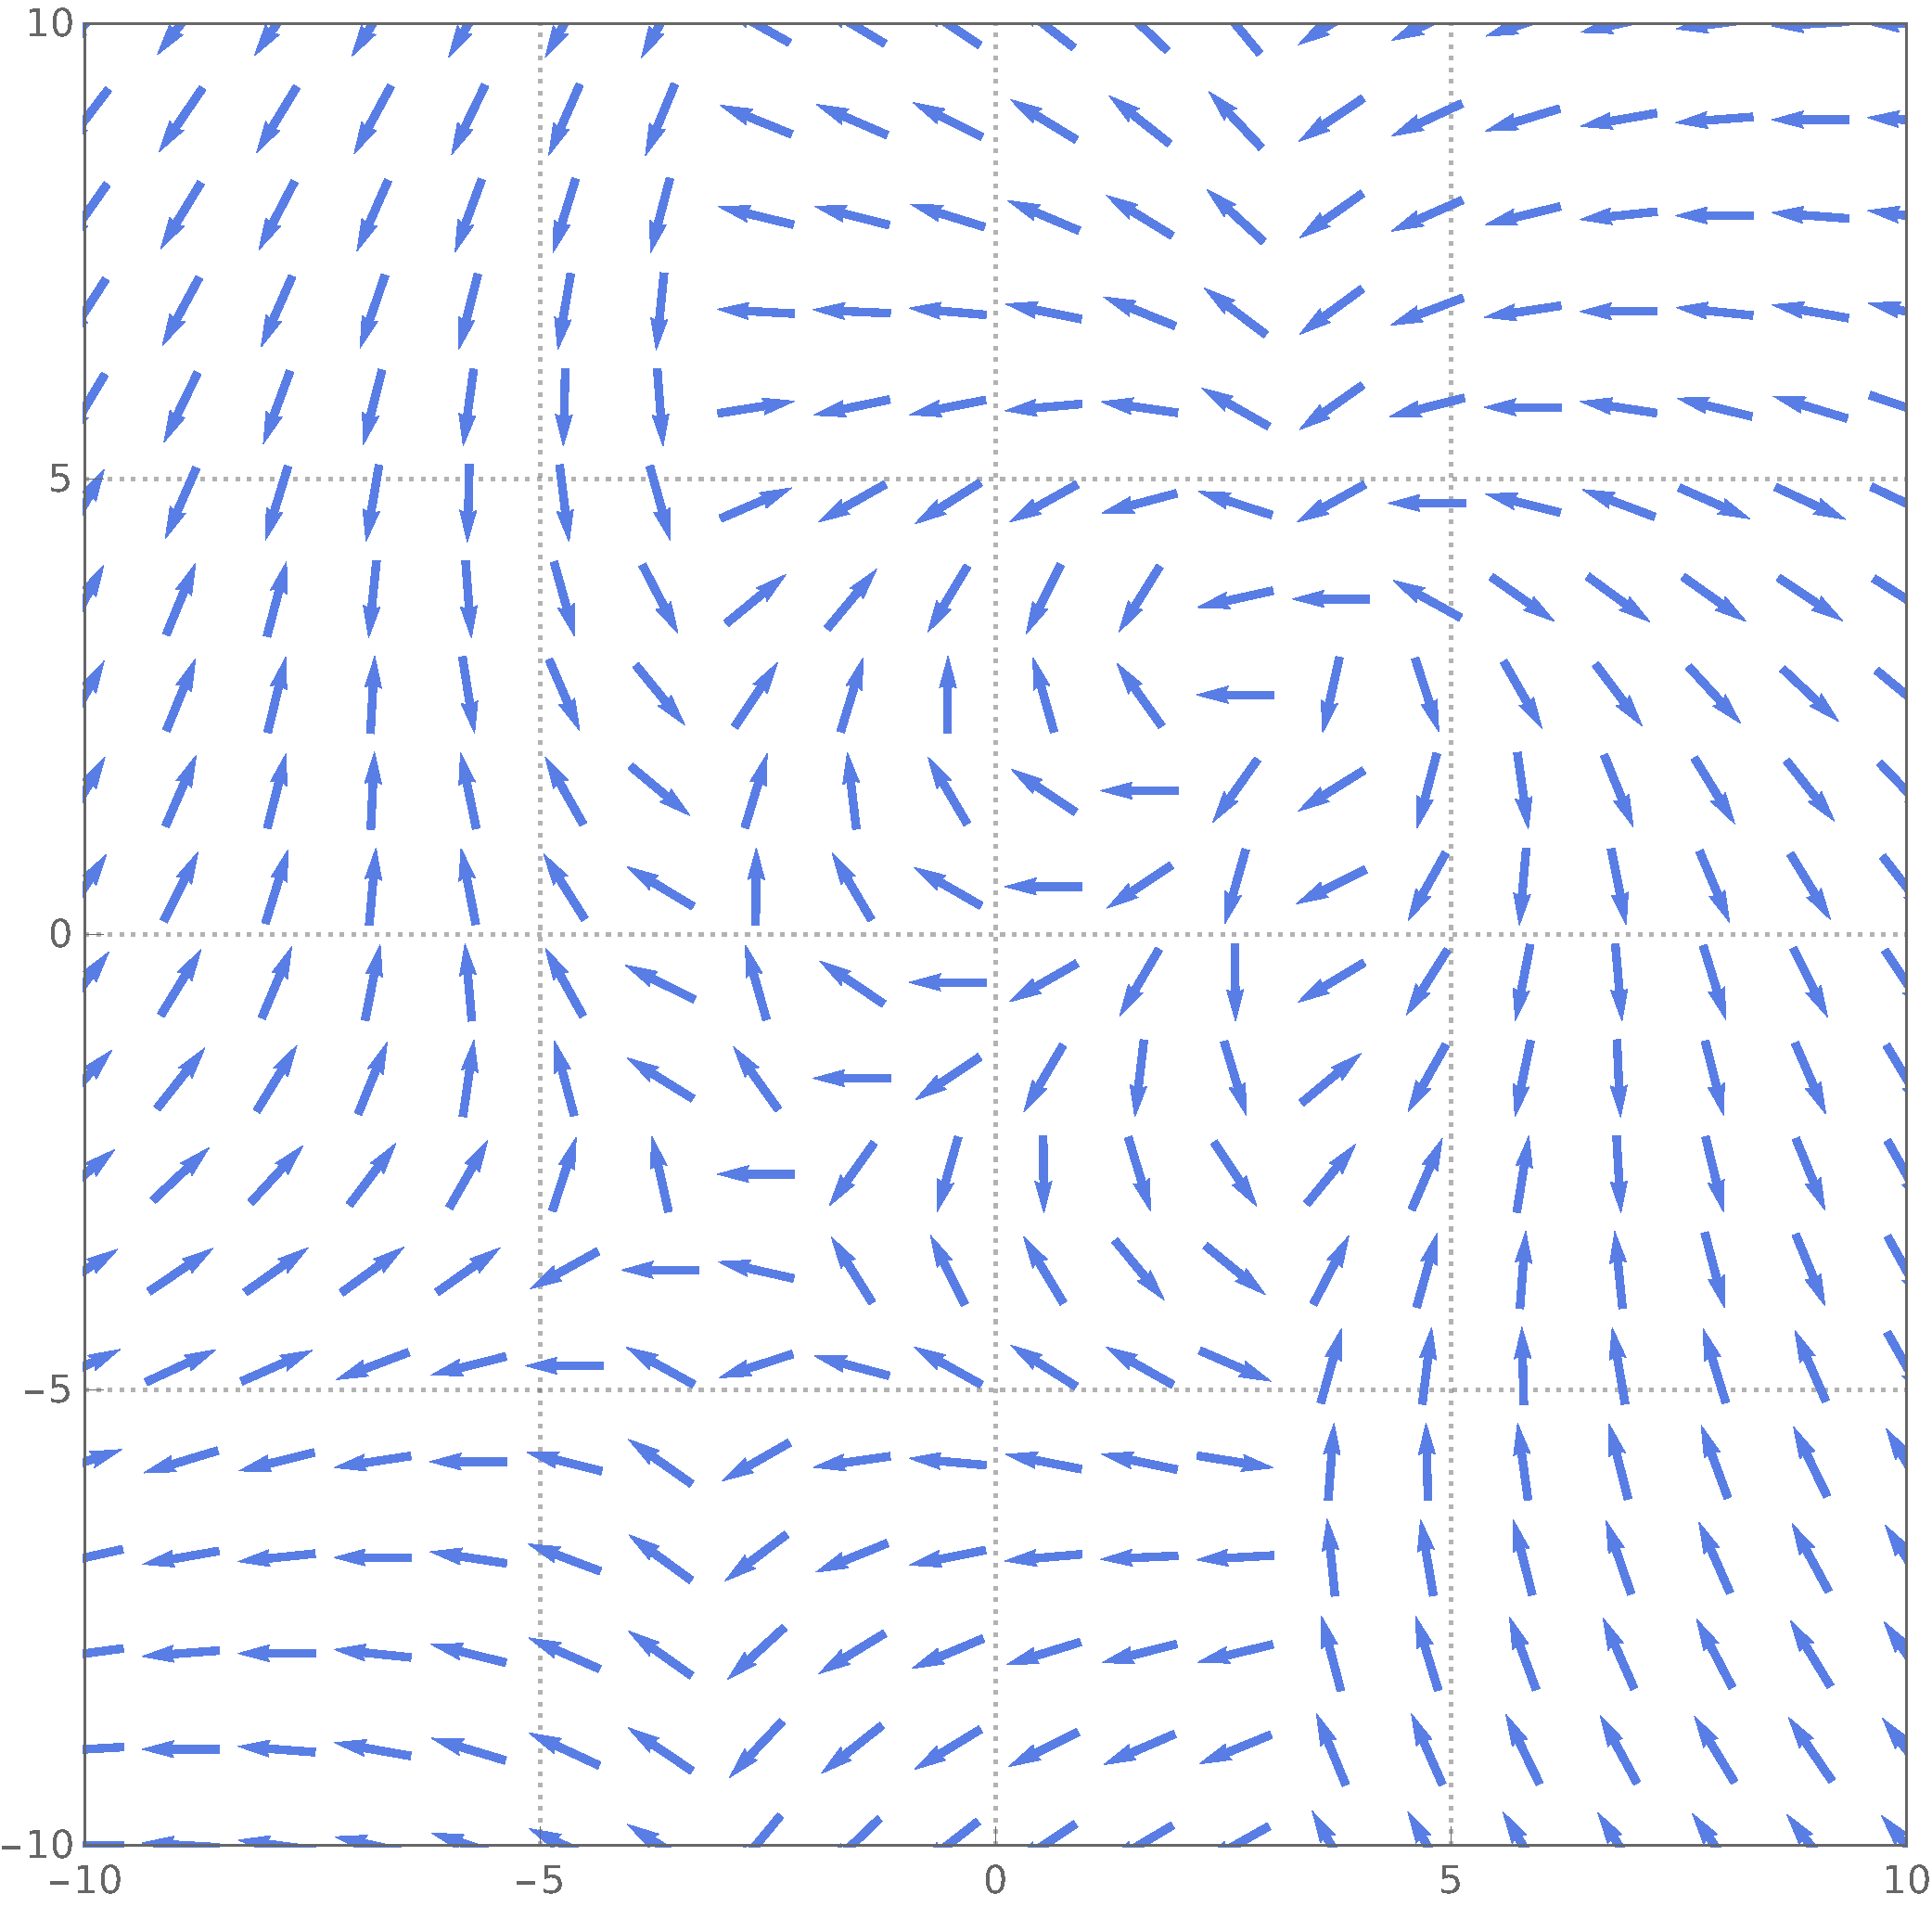
\includegraphics[scale=0.2]{spin.pdf}
			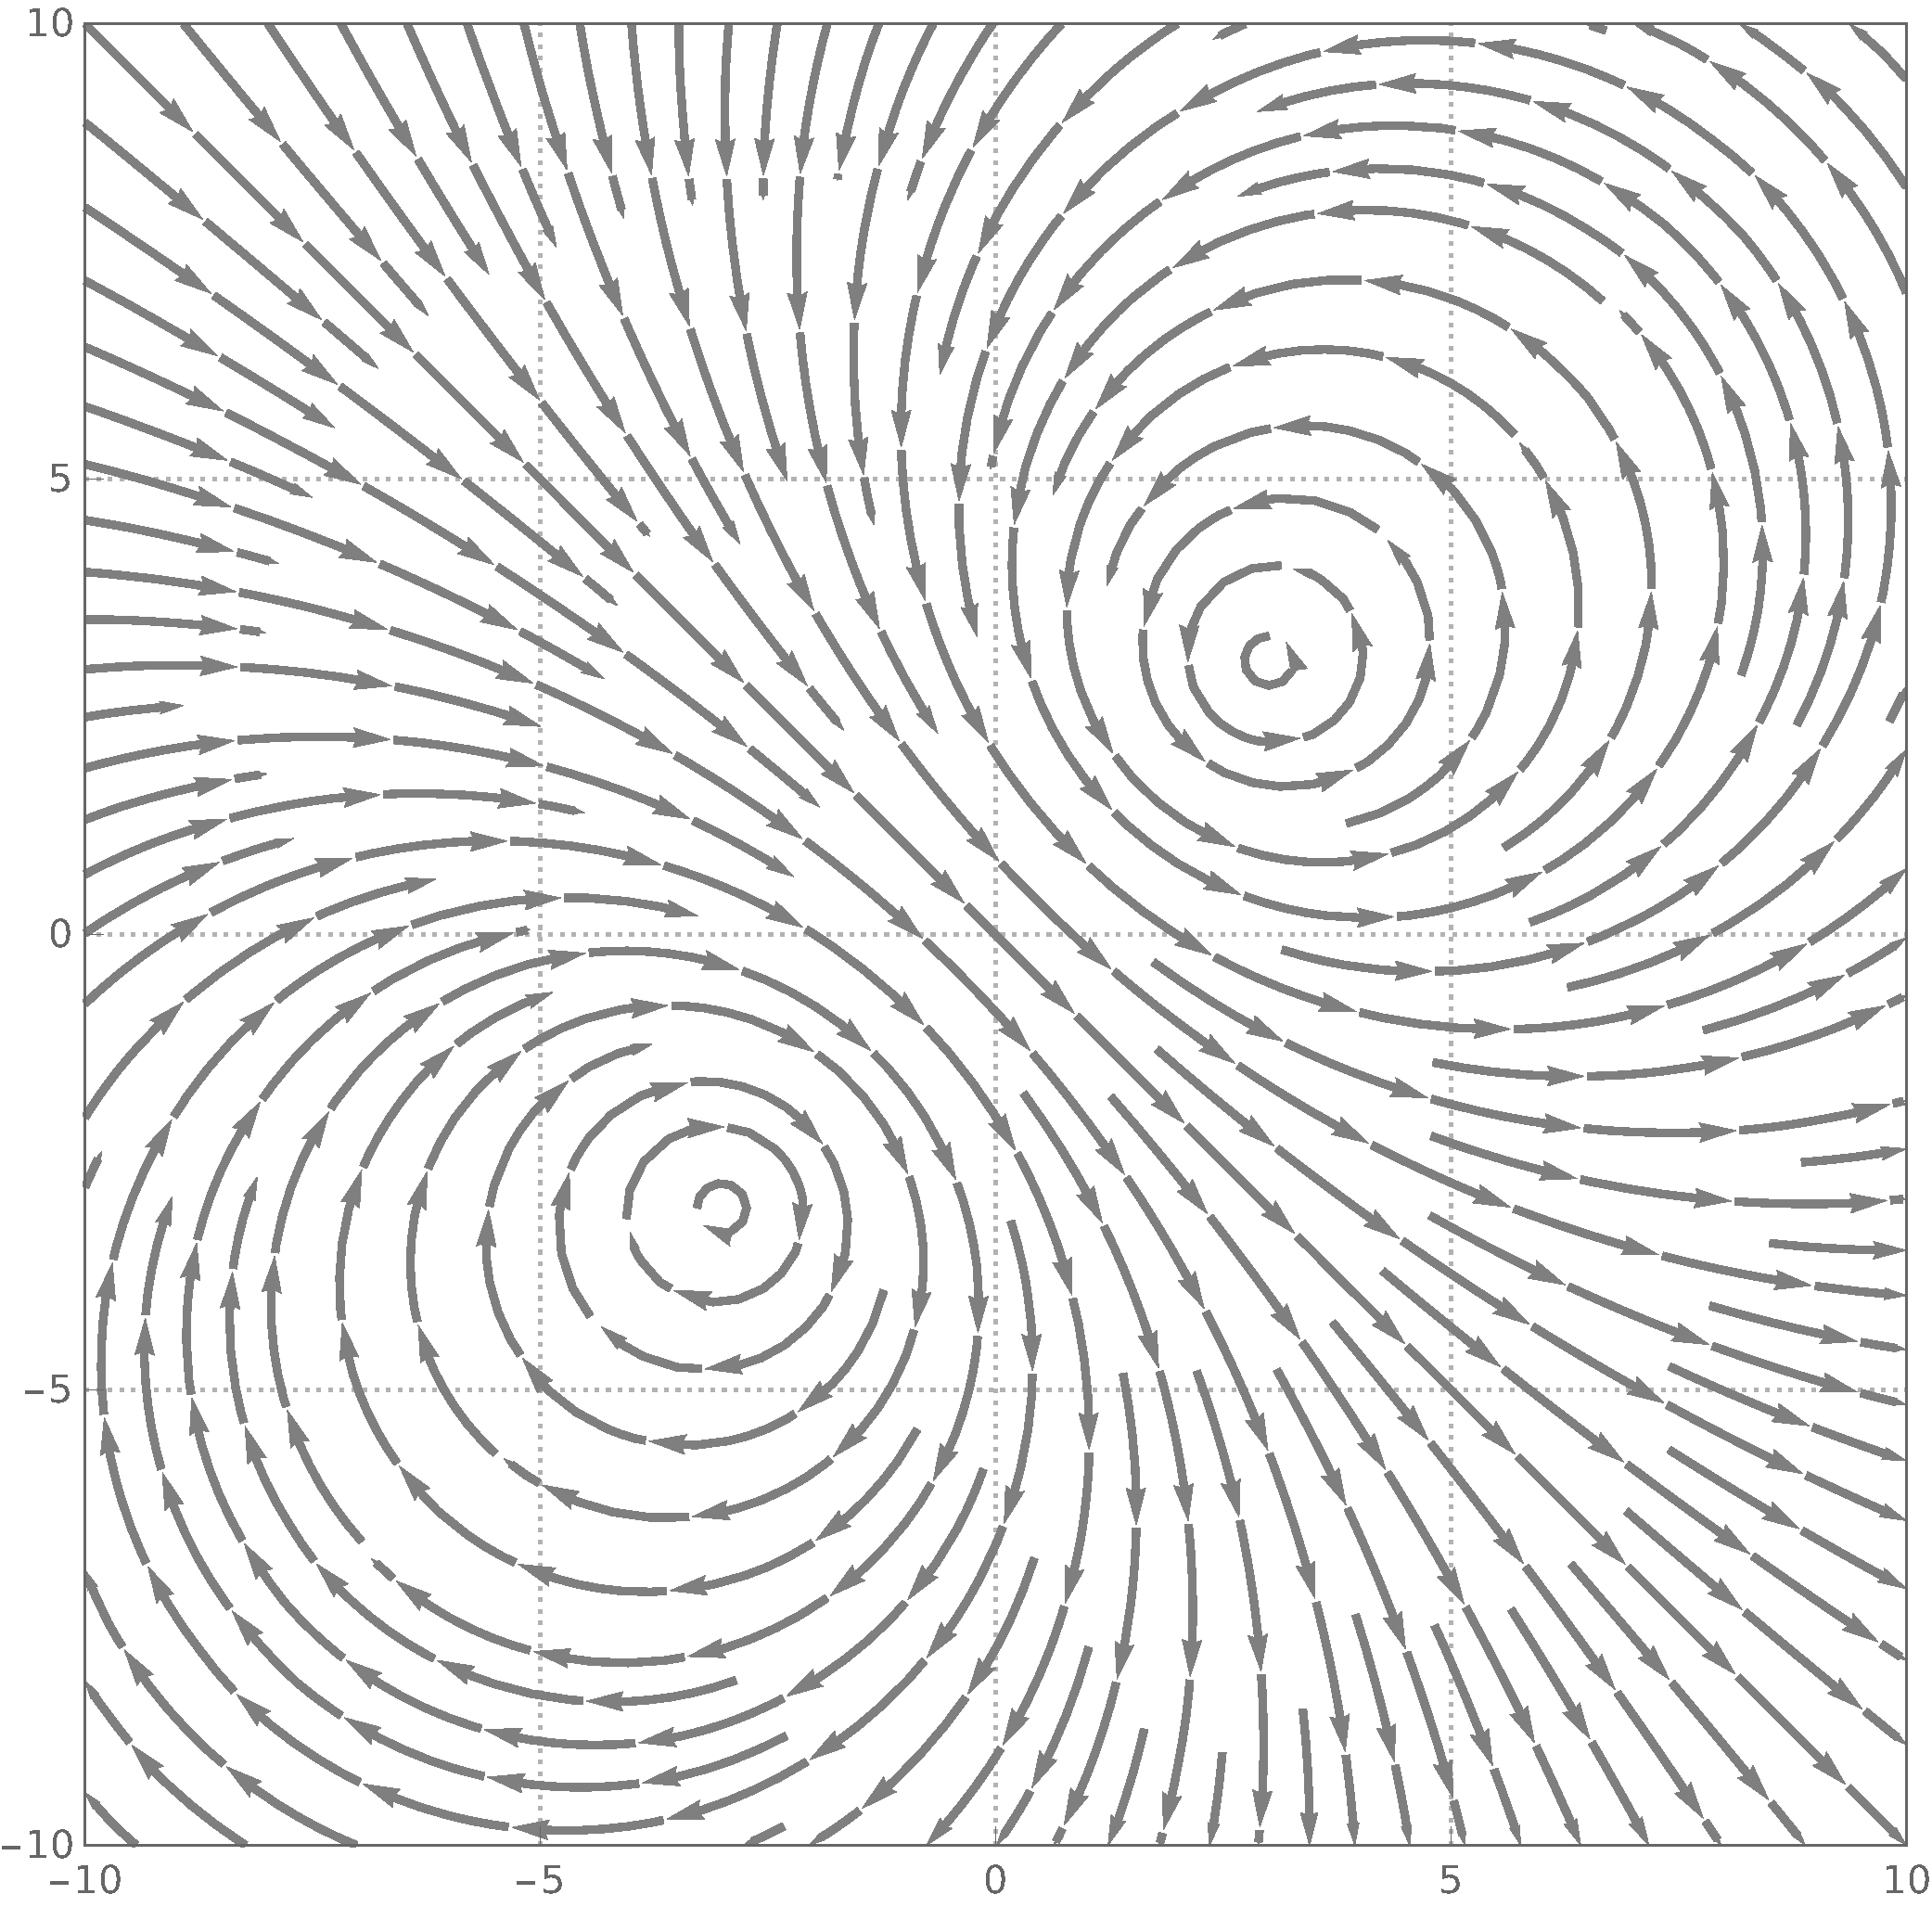
\includegraphics[scale=0.2]{vector.pdf}
			\caption{{\bf One vortex/Antivortex Pairs at Confined Phase}: Spin configuration $\theta_i$ for vortex (or topological defects) configurations $\theta(\bm{r})=N\arctan\dfrac{y-y_0}{x-x_0}$ with opposite topological charges $N=3$ locating at $(x_0,y_0)=(3,3)$ and $(x_0,y_0)=(-3,-3)$ on a $10\times 10$ squre lattice and the corresponding stream lines of vector fields $\bm{v}\equiv\nabla\theta(\bm{r})$.}
			\label{fig:1}
		\end{figure}
		\textbf{But if temperature is raised above the critical point, not only will vortex/antivortex pairs proliferate, the interaction-induced bonds between will melt down, creating isolate topological charges bahaving like itinerate positive/negative electric charges}. Such phase is called \emph{deconfined phase}. FIG. \ref{fig:2} is an illustration of three meltdown bound states. It is clear that proliferation of deconfined pairs will reduce the correlation of spins. So it's reasonable to have a exponential-decay behavior of correlation function and a finite correlation length at high temperature.
		\begin{figure}[!htp]
			\centering
			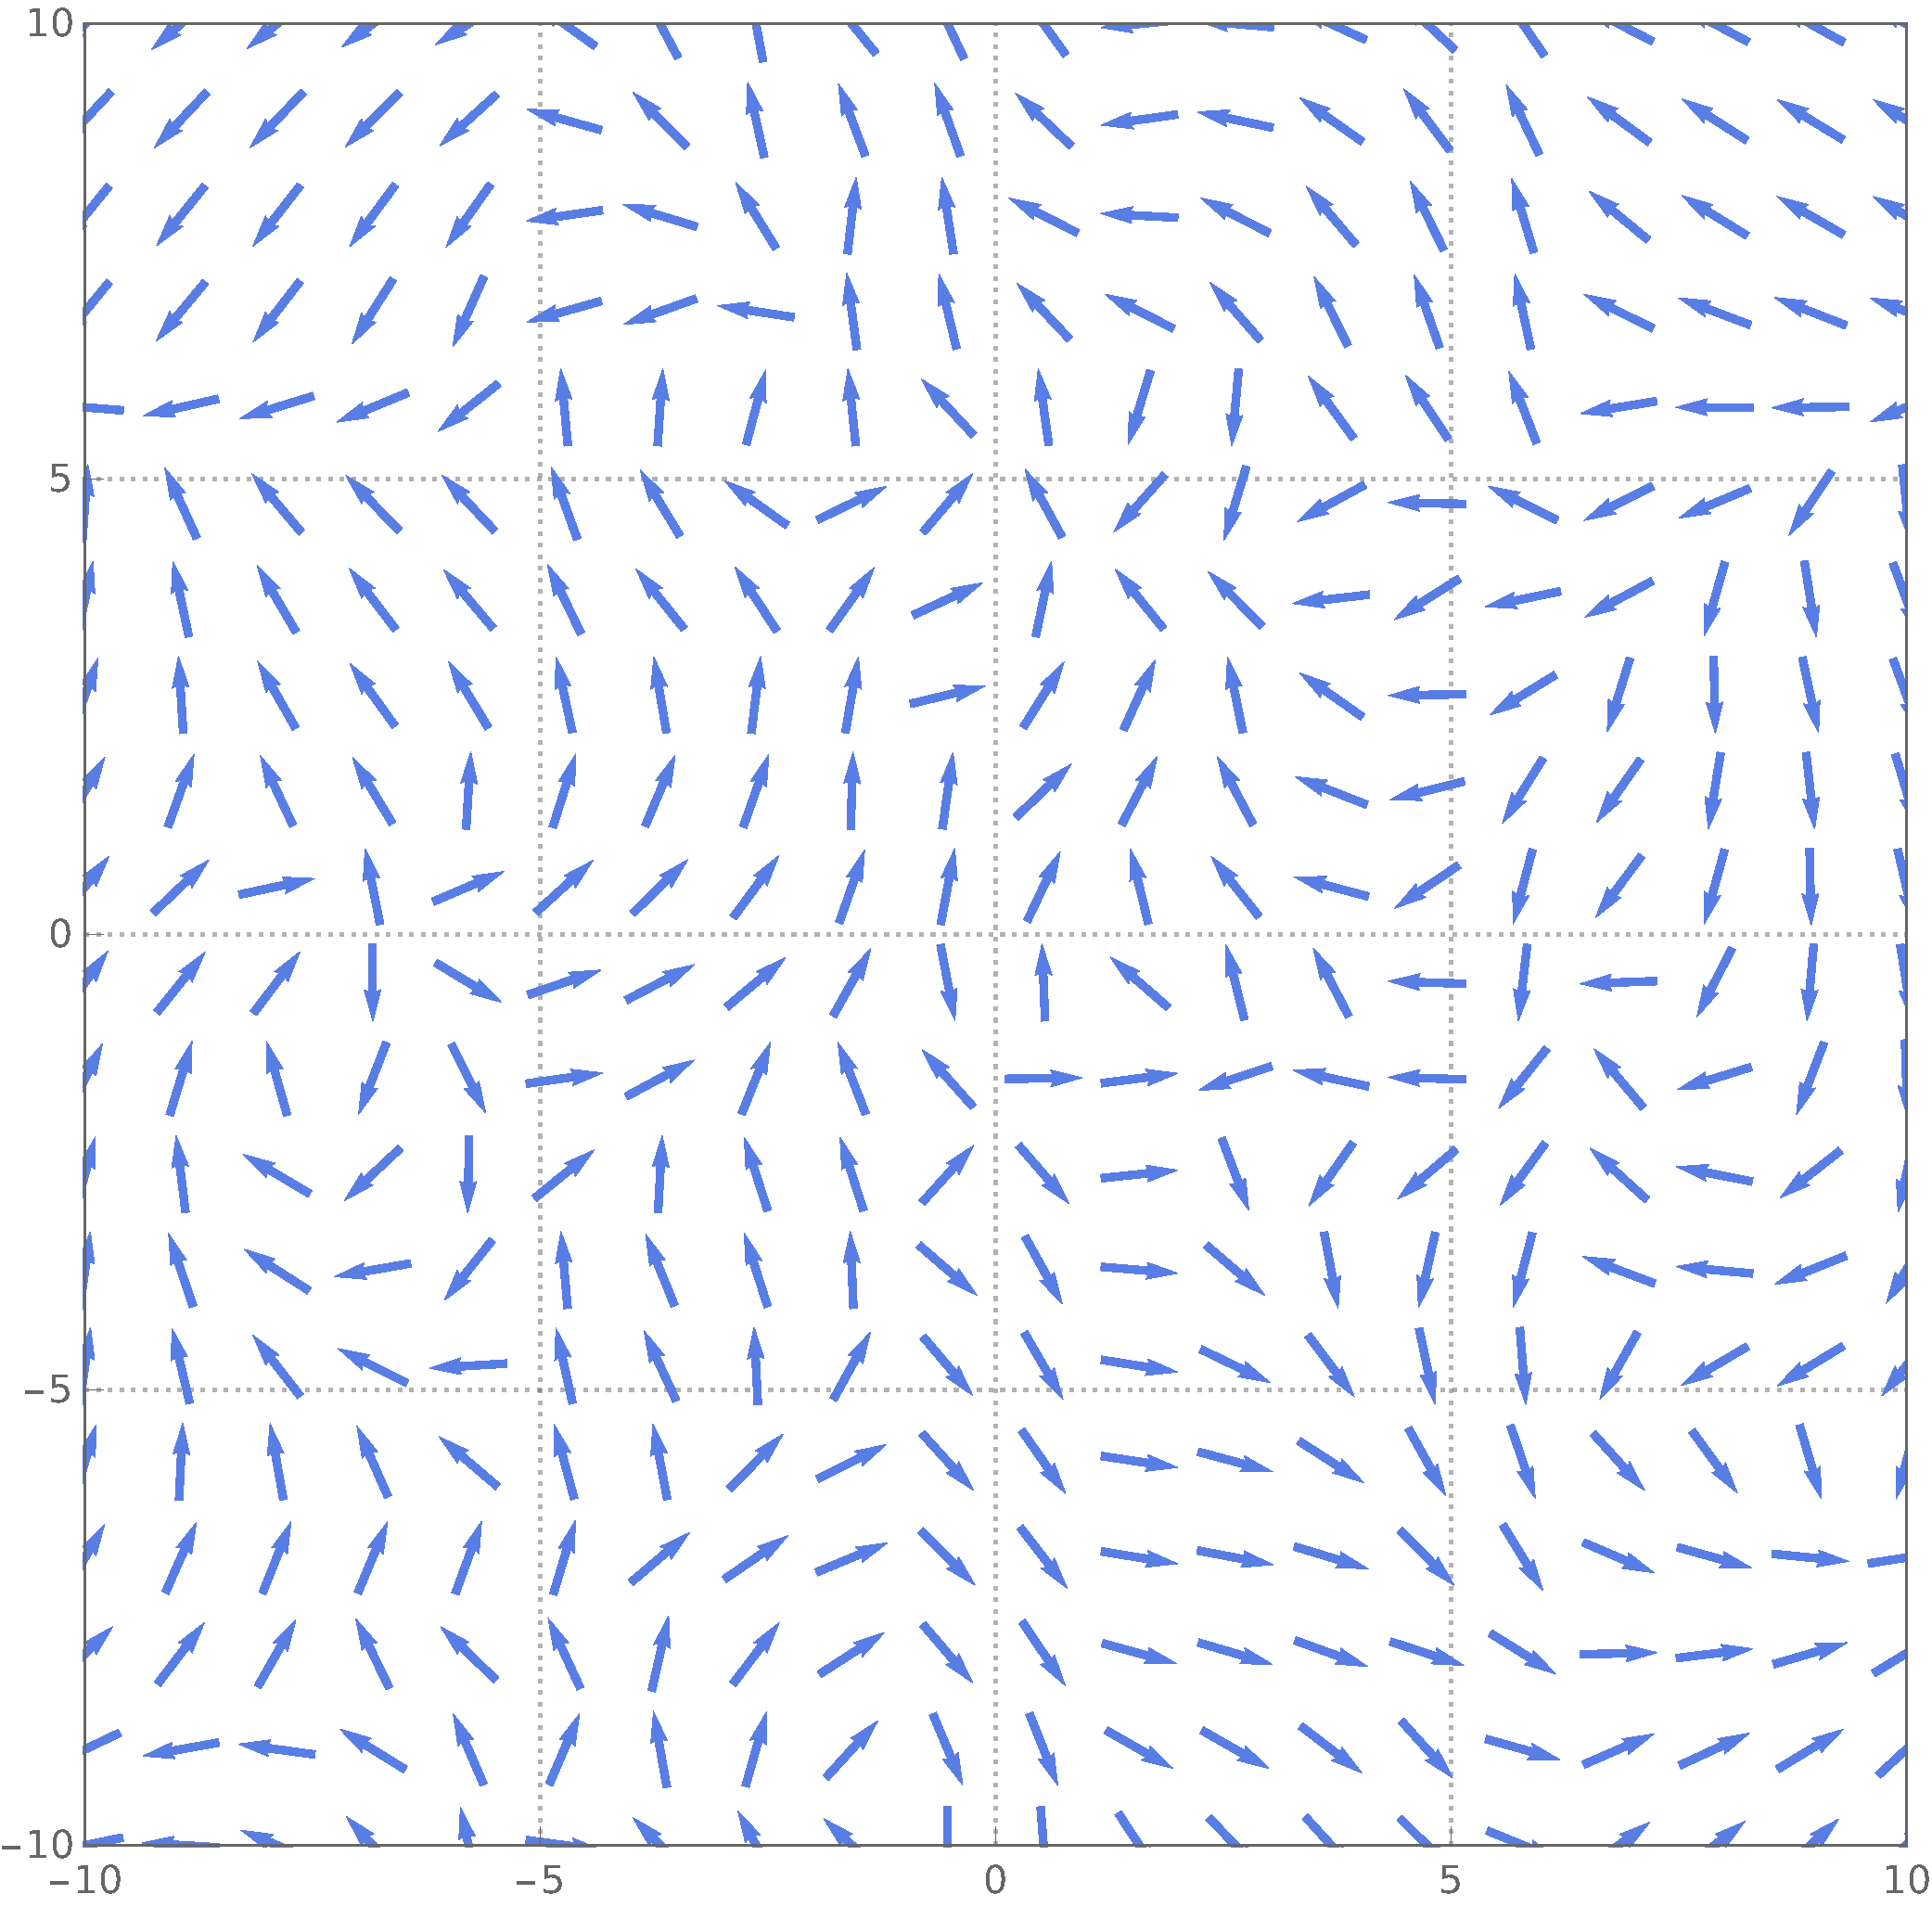
\includegraphics[scale=0.2]{spin2.pdf}
			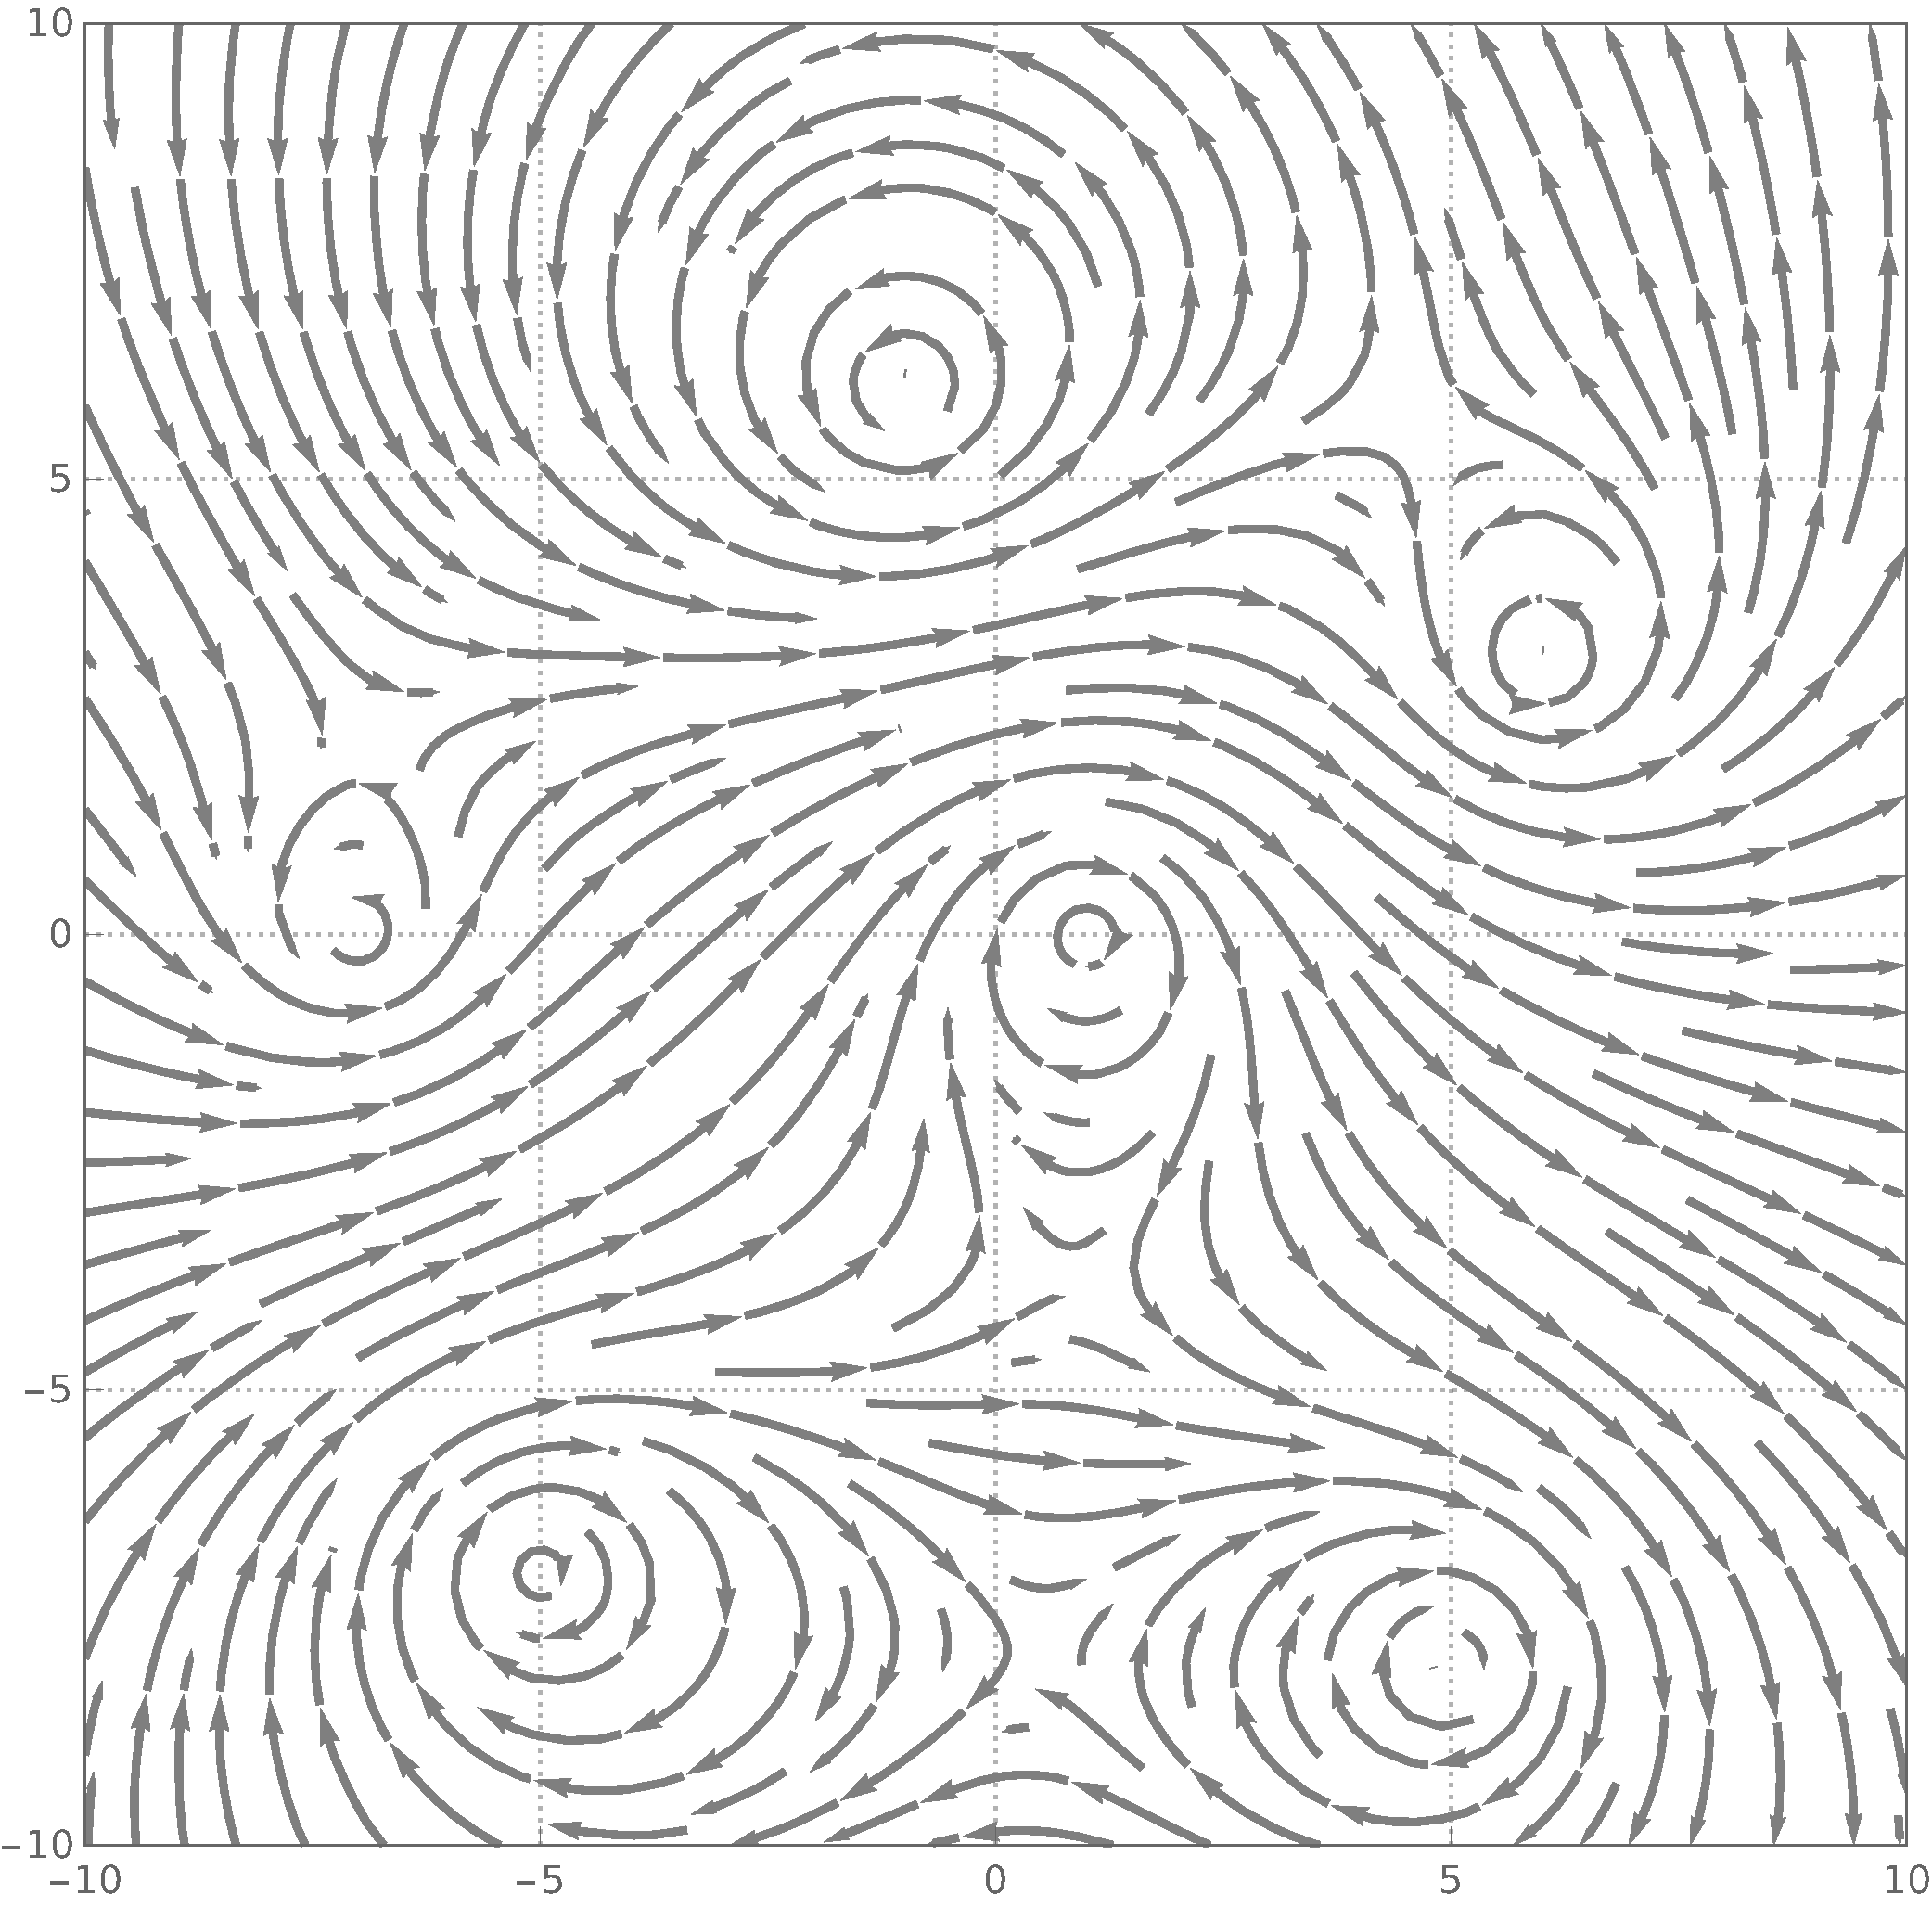
\includegraphics[scale=0.2]{vector2.pdf}
			\caption{{\bf Proliferation and Breakdown of Vortex/Antivortex Pairs at Deconfined Phase}: Breakdown of three pairs of vortex/antivotex bonds with topological charge $N=2,3,4$.}
			\label{fig:2}
		\end{figure}
		
		

	\subsection{Duality to Sine-Gordon Model}
		Ignoring the unimportant spin-wave part of partition function, something magic will happen if the left part going back to continuum limit. First of all, since charge neutrality tells us $\sum_{m}\sum_{\bm{r}}m(\bm{r})\equiv0$, quadratic terms in \eqref{2.1.7} at independent position actually have no contribution
		\begin{equation*}
			\Z_{vor}=\sum_{m(\bm{r})=-\infty}^\infty\exp \left\{-\dfrac{\pi^2\beta J}{2}\sum_{\bm{r}}m^2(\bm{r})+\pi\beta J\sum_{\bm{r}\neq\bm{r'}}m(\bm{r})\ln\left(\dfrac{|\bm{r'}-\bm{r}|}{a}\right)m(\bm{r'})\right\}.
		\end{equation*}
		Defining the \emph{fugacity} $y\equiv e^{-\beta J\pi^2/2}$, and recovering logarithmic term with Gaussian integral over some continuous scalar field $\varphi(\bm{r})$, then
		\begin{equation}\label{2.2.1}
			\Z_{vor}=\prod_{\bm{r}}\int\dd\varphi(\bm{r})\sum_{m(\bm{r})=-\infty}^\infty\exp \left\{\ln y\sum_{\bm{r}}m^2(\bm{r})-\dfrac{1}{2\beta J}\sum_{\bm{r},\mu}(\nabla\varphi)^2+2\pi i\sum_{\bm{r}}m(\bm{r})\right\}.
		\end{equation}
		Remember that we are working in low-temperature limit, or $\ln y \rightarrow -\infty$, therefore the expression of $m(\bm{r})$ in the exponent of \eqref{2.2.1} will be highly dominated by the quadratic term. And because $\ln y$ is negative, only small $m(\bm{r})$ terms will have non-vanishing contribution in the vortex partition function. So we can effectively truncate the summation at configuration $m=0,\pm1$, obtaining
		\begin{align}
		 	\Z_{vor}&=\prod_{\bm{r}}\int\dd\varphi(\bm{r})\exp \left\{-\dfrac{1}{2\beta J}\sum_{\bm{r},\mu}(\nabla\varphi)^2\right\}\times\prod_{\bm{r}}\sum_{m(\bm{r})=-1}^{+1}\exp \bigg\{\ln y\cdot m^2(\bm{r})+2\pi im(\bm{r})\bigg\}\nonumber\\
		 	&=\prod_{\bm{r}}\int\dd\varphi(\bm{r})\exp \left\{-\dfrac{1}{2\beta J}\sum_{\bm{r},\mu}(\nabla\varphi)^2\right\}\times \prod_{\bm{r}}\bigg(1+2y\cos(2\pi\varphi(\bm{r}))\bigg)\nonumber\\
		 	&=\prod_{\bm{r}}\int\dd\varphi(\bm{r})\exp \left\{-\dfrac{1}{2\beta J}\sum_{\bm{r},\mu}(\nabla\varphi)^2\right\}\times \exp\left\{\sum_{\bm{r}}2y\cos(2\pi\varphi(\bm{r}))\right\}.\label{2.2.2}
		 \end{align}
		 Rescaling $\varphi(\bm{r})\mapsto\sqrt{\beta J}\varphi(\bm{r})$ and working in continuum limit, we finally come to the celebrated universal class of renormalization group---\emph{sine-Gordon model}
		\begin{equation}\label{2.2.3}
			\Z_{vor}=\int\mathcal{D}\varphi\,\exp \left\{-\int\dd\bm{r} \left[\dfrac{1}{2}(\nabla\varphi(\bm{r}))^2-2y\cos\left(2\pi\sqrt{\beta J}\varphi(\bm{r})\right)\right]\right\}.
		\end{equation}
		Clearly after this duality mapping our system now possesses discrete symmetry $\varphi(\bm{r})\mapsto \varphi(\bm{r})+m/\sqrt{\beta J}$ for all $m\in\mathbb{Z}$. If you identify each $\varphi(\bm{r})$ with origianl compact angle field $\theta(\bm{r})$ with stereographic projection, then second term above can be explained as, \textbf{\color{red} due to self-interaction of instantons, $U(1)$ symmetry in XY model breaks down to $\mathbb{Z}_{m/\sqrt{\beta J}}$ symmetry in Sine-Gordon model}.


\section{Renormalization Group}
	We will mainly follow momentum-shell renormalization group analysis in  \cite{kogut1979introduction,nagaosa2013quantum} will little change, so I shall not ``re-invent the wheel'' in my note. Although subtle techniques of $\varepsilon$-expansion \cite{wilson1974renormalization} are unavoidable for single-loop calculation, we will not waste time on such details. Maybe we will go back to this example with much more advanced, elegant and systematic treatments of conformal invanriance around critical region.


\section{A Rush Course on Conformal Field Theory}
\iffalse
	We start from the free massless bosonic fields $\phi(\sigma^0,\sigma^1)$ on a flat \emph{Euclidiean} spacetime $\gamma_{\mu\nu}=\delta_{\mu\nu}$
	\begin{equation}\label{2.1}
		S[\phi]\equiv\dfrac{1}{4\pi g}\int\mathrm{vol}\,\partial_\mu\phi \partial^\mu\phi=\dfrac{1}{4\pi g}\int\dd^2\sigma\,\partial_\mu\phi \partial ^\mu\phi
	\end{equation}
	where the volume form (on the world sheet) is simply 
	\begin{equation*}
		\mathrm{vol}=\sqrt{|\gamma|}\dd\sigma^0\wedge\dd\sigma^1=\dd\sigma^0\wedge\dd\sigma^1.
	\end{equation*}
	Since $\mathbb{R}^2$ is isomorphic to $\mathbb{C}$, it's convenient to work on the complex plane $(z^0,z^1)\equiv(z,\bar z)$ to decoupling two variables
	\begin{equation*}
		z\equiv \sigma^0+i\sigma^1,\quad \bar z\equiv\sigma^0-i\sigma^1.
	\end{equation*}
	Then the metric becomes
	\begin{equation*}
		g_{\mu\nu}=\dfrac{\partial \sigma^\rho}{\partial z^\mu}\dfrac{\partial \sigma^\lambda}{\partial z^\nu}\gamma_{\rho\lambda}=\left(\begin{array}{cc}
			0 & \frac12\\ \frac12 & 0
		\end{array}\right)
	\end{equation*}
	and action \eqref{2.1} becomes
	\begin{equation}\label{2.2}
		S[\phi]=\dfrac{1}{4\pi g}\int\dfrac{1}{2}\dd z\wedge\dd\bar z\, \partial_\mu\phi \partial^\mu\phi=
	\end{equation}

\section{Application to Sine-Gordon Model}

\fi


\bibliography{hxd}
\bibliographystyle{apsrev} % apsrev is format for PRL of APS
\end{document}